% !TEX root = presentation.tex
%LTeX: language=de-CH

% \section{Einleitung}

\begin{frame}
  \frametitle{Forecast: 01-May-2025 at 00:00, Level 850 hPa}
  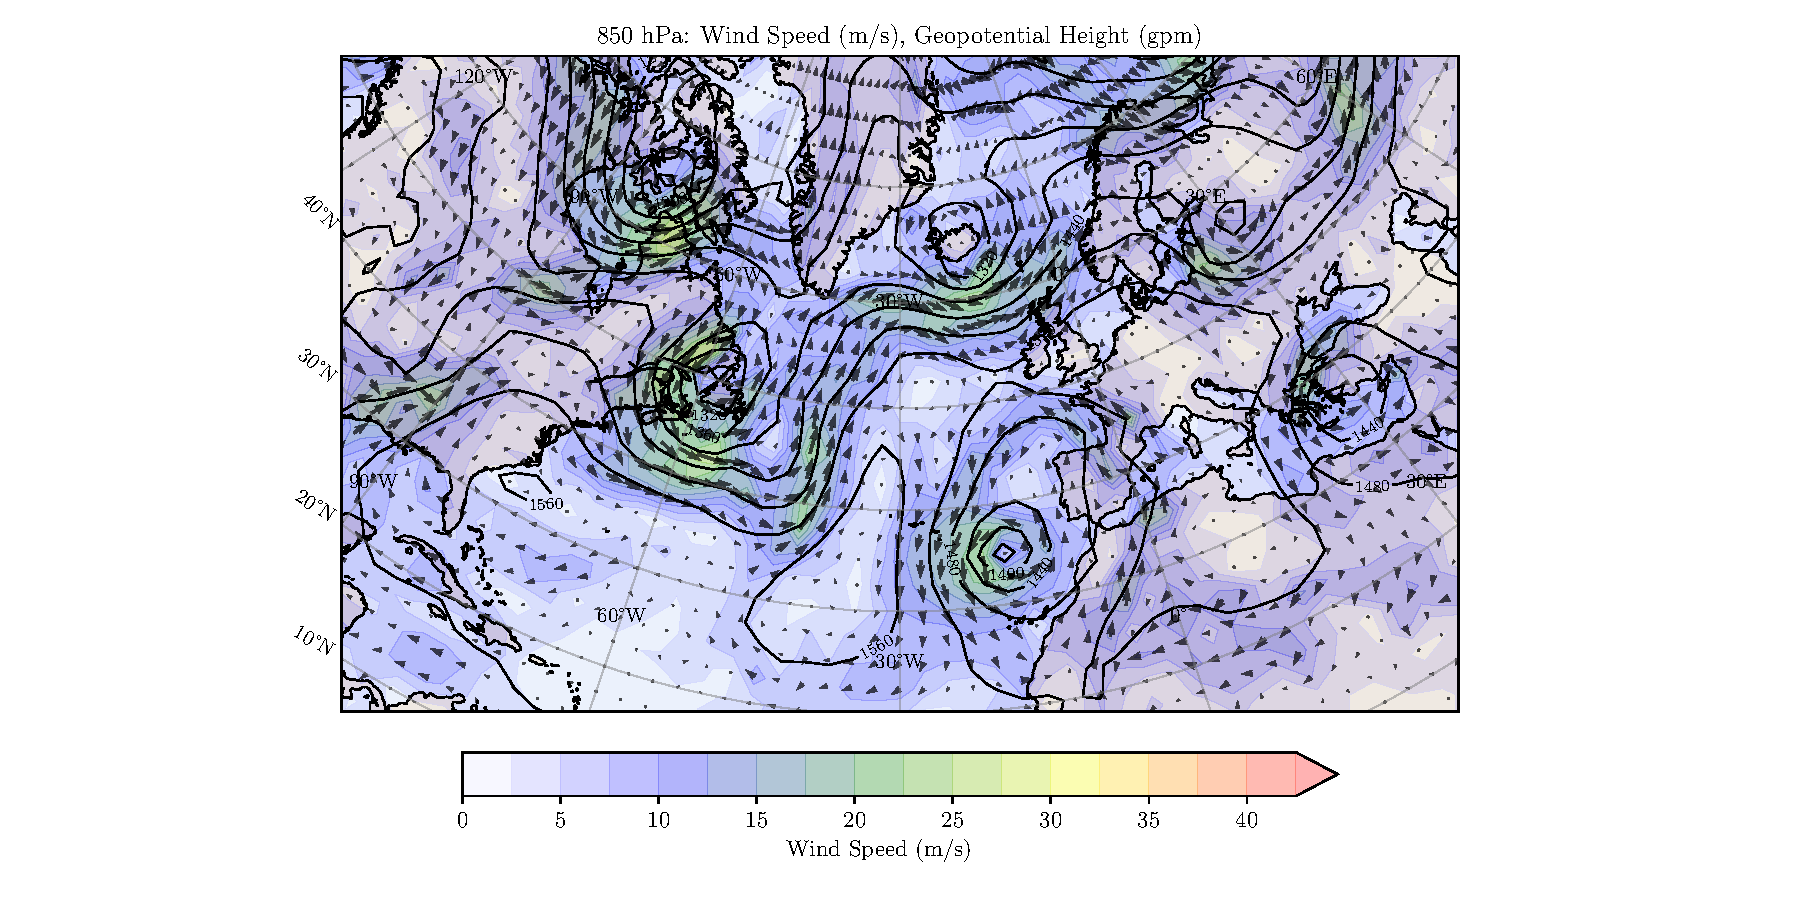
\includegraphics[width=\textwidth]{../images/weather/data_2025_5_1_00:00_850.pdf}
\end{frame}
\begin{frame}
  \frametitle{Forecast: 01-May-2025 at 00:00, Level 500 hPa}
  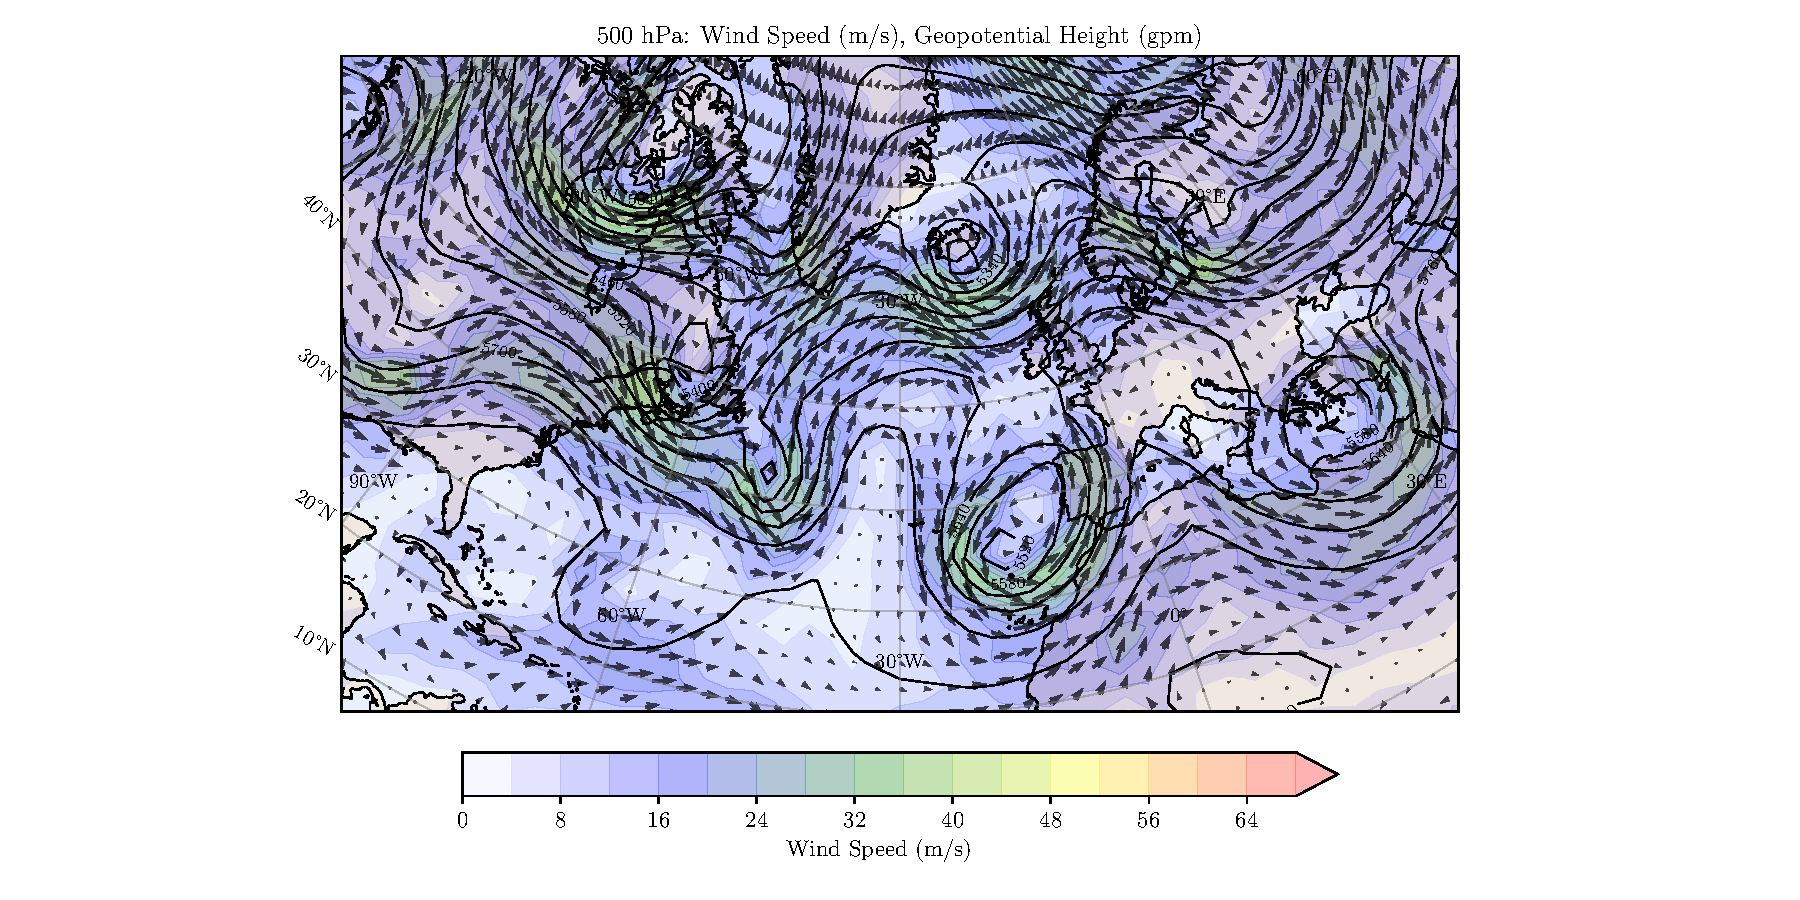
\includegraphics[width=\textwidth]{../images/weather/data_2025_5_1_00:00_500.pdf}
\end{frame}
\begin{frame}
  \frametitle{Forecast: 01-May-2025 at 00:00, Level 200 hPa}
  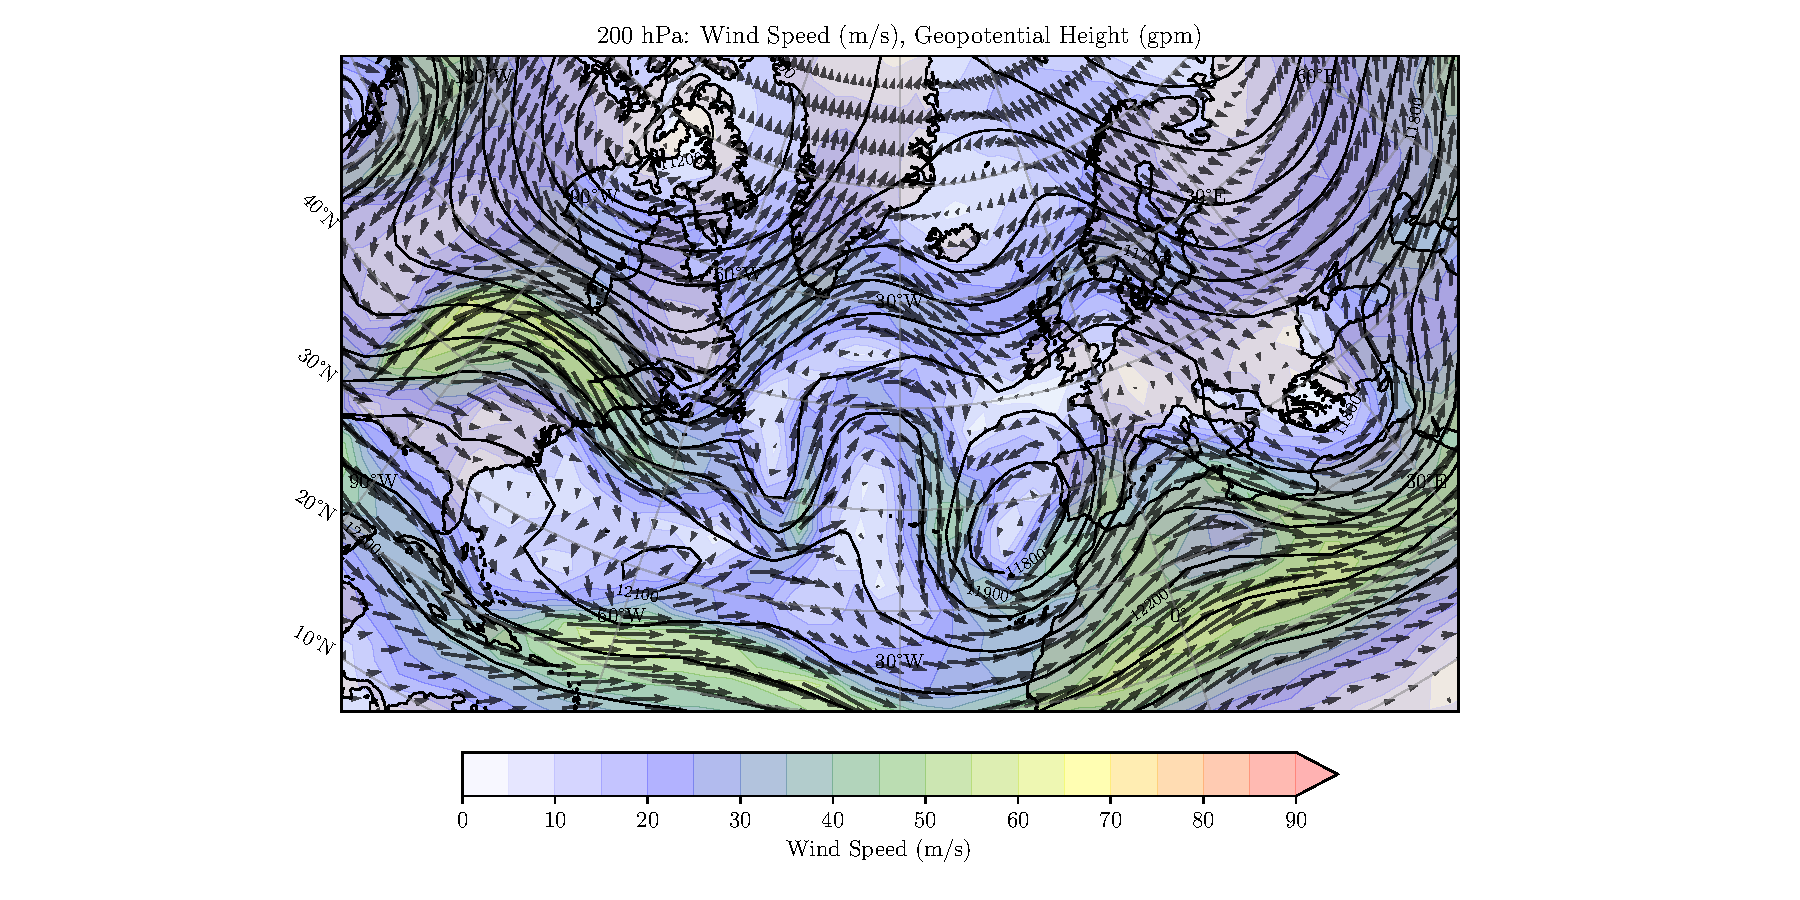
\includegraphics[width=\textwidth]{../images/weather/data_2025_5_1_00:00_200.pdf}
\end{frame}

% In your document body:

\foreach \level in {500} {
  \foreach \day in {1,...,10} {
    \foreach \time in {00:00,12:00} {
      \begin{frame}
        \frametitle{Forecast: \day-May-2025 at \time, Level \level hPa}
        \includegraphics[width=\textwidth]{../images/weather/data_2025_5_\day_\time_\level.png}
      \end{frame}
    }
  }
}



% In your document body:
\foreach \level in {500} {
\foreach \day in {1,...,10} {
  \foreach \time in {00:00,12:00} {
      \begin{frame}[plain]
        \frametitle{Forecast: \day-May-2025 at \time, Level \level hPa}
        \begin{center}
          \includegraphics[width=0.5\textwidth]{../images/weather/data_2025_5_\day_\time_\level_polar.png}
        \end{center}
      \end{frame}
    }
  }
}

% In your document body:
\foreach \level in {500} {
\foreach \day in {20,...,31} {
  \foreach \time in {12:00} {
      \begin{frame}[plain]
        \frametitle{Forecast: \day-July-2010 at \time, Level \level hPa}
        \begin{center}
          \includegraphics[width=0.5\textwidth]{../images/weather/data_2010_7_\day_\time_\level_polar.png}
        \end{center}
      \end{frame}
    }
  }
}

\foreach \level in {500} {
\foreach \day in {1,...,10} {
  \foreach \time in {12:00} {
      \begin{frame}[plain]
        \frametitle{Forecast: \day-August-2010 at \time, Level \level hPa}
        \begin{center}
          \includegraphics[width=0.5\textwidth]{../images/weather/data_2010_8_\day_\time_\level_polar.png}
        \end{center}
      \end{frame}
    }
  }
}

\foreach \level in {500} {
\foreach \day in {20,...,31} {
  \foreach \time in {12:00} {
      \begin{frame}[plain]
        \frametitle{Forecast: \day-July-2010 at \time, Level \level hPa}
        \begin{center}
          \includegraphics[width=\textwidth]{../images/weather/data_2010_7_\day_\time_\level.png}
        \end{center}
      \end{frame}
    }
  }
}

\foreach \level in {500} {
\foreach \day in {1,...,10} {
  \foreach \time in {12:00} {
      \begin{frame}[plain]
        \frametitle{Forecast: \day-August-2010 at \time, Level \level hPa}
        \begin{center}
          \includegraphics[width=\textwidth]{../images/weather/data_2010_8_\day_\time_\level.png}
        \end{center}
      \end{frame}
    }
  }
}